\documentclass[12pt]{article}\usepackage[]{graphicx}\usepackage[]{color}
%% maxwidth is the original width if it is less than linewidth
%% otherwise use linewidth (to make sure the graphics do not exceed the margin)
\makeatletter
\def\maxwidth{ %
  \ifdim\Gin@nat@width>\linewidth
    \linewidth
  \else
    \Gin@nat@width
  \fi
}
\makeatother

\definecolor{fgcolor}{rgb}{0.345, 0.345, 0.345}
\newcommand{\hlnum}[1]{\textcolor[rgb]{0.686,0.059,0.569}{#1}}%
\newcommand{\hlstr}[1]{\textcolor[rgb]{0.192,0.494,0.8}{#1}}%
\newcommand{\hlcom}[1]{\textcolor[rgb]{0.678,0.584,0.686}{\textit{#1}}}%
\newcommand{\hlopt}[1]{\textcolor[rgb]{0,0,0}{#1}}%
\newcommand{\hlstd}[1]{\textcolor[rgb]{0.345,0.345,0.345}{#1}}%
\newcommand{\hlkwa}[1]{\textcolor[rgb]{0.161,0.373,0.58}{\textbf{#1}}}%
\newcommand{\hlkwb}[1]{\textcolor[rgb]{0.69,0.353,0.396}{#1}}%
\newcommand{\hlkwc}[1]{\textcolor[rgb]{0.333,0.667,0.333}{#1}}%
\newcommand{\hlkwd}[1]{\textcolor[rgb]{0.737,0.353,0.396}{\textbf{#1}}}%
\let\hlipl\hlkwb

\usepackage{framed}
\makeatletter
\newenvironment{kframe}{%
 \def\at@end@of@kframe{}%
 \ifinner\ifhmode%
  \def\at@end@of@kframe{\end{minipage}}%
  \begin{minipage}{\columnwidth}%
 \fi\fi%
 \def\FrameCommand##1{\hskip\@totalleftmargin \hskip-\fboxsep
 \colorbox{shadecolor}{##1}\hskip-\fboxsep
     % There is no \\@totalrightmargin, so:
     \hskip-\linewidth \hskip-\@totalleftmargin \hskip\columnwidth}%
 \MakeFramed {\advance\hsize-\width
   \@totalleftmargin\z@ \linewidth\hsize
   \@setminipage}}%
 {\par\unskip\endMakeFramed%
 \at@end@of@kframe}
\makeatother

\definecolor{shadecolor}{rgb}{.97, .97, .97}
\definecolor{messagecolor}{rgb}{0, 0, 0}
\definecolor{warningcolor}{rgb}{1, 0, 1}
\definecolor{errorcolor}{rgb}{1, 0, 0}
\newenvironment{knitrout}{}{} % an empty environment to be redefined in TeX

\usepackage{alltt}

\usepackage{fullpage,amsmath,amsthm,framed,fancyhdr,amsfonts,graphicx,color,titlesec,enumitem,rotating,hyperref}
\usepackage[margin=1in]{geometry}
\usepackage[labelfont=bf,labelsep=period]{caption}

%%%%% PLACE YOUR OWN MACROS HERE %%%%%

%%%%%%%%%%%%%%%%%%%%%%%%%%
%  Bold Digits           %
%%%%%%%%%%%%%%%%%%%%%%%%%%
%
%
\def\bzero{{\bf 0}}
\def\bone{{\bf 1}}
%
%
%%%%%%%%%%%%%%%%%%%%%%%%%%
%  Bold Roman Letters    %
%%%%%%%%%%%%%%%%%%%%%%%%%%
%
%
\def\ba{{\mbox{\bmath$a$}}}
\def\bb{{\bf b}}
\def\bc{{\bf c}}
\def\bd{{\bf d}}
\def\be{{\bf e}}
\def\bdf{{\bf f}}
\def\bg{{\mbox{\bmath$g$}}}
\def\bh{{\bf h}}
\def\bi{{\bf i}}
\def\bj{{\bf j}}
\def\bk{{\bf k}}
\def\bl{{\bf l}}
\def\bm{{\bf m}}
\def\bn{{\bf n}}
\def\bo{{\bf o}}
\def\bp{{\bf p}}
\def\bq{{\bf q}}
\def\br{{\bf r}}
\def\bs{{\bf s}}
\def\bt{{\bf t}}
\def\bu{{\bf u}}
\def\bv{{\bf v}}
\def\bw{{\bf w}}
\def\bx{{\bf x}}
\def\by{{\bf y}}
\def\bz{{\bf z}}
\def\bA{{\bf A}}
\def\bB{{\bf B}}
\def\bC{{\bf C}}
\def\bD{{\bf D}}
\def\bE{{\bf E}}
\def\bF{{\bf F}}
\def\bG{{\bf G}}
\def\bH{{\bf H}}
\def\bI{{\bf I}}
\def\bJ{{\bf J}}
\def\bK{{\bf K}}
\def\bL{{\bf L}}
\def\bM{{\bf M}}
\def\bN{{\bf N}}
\def\bO{{\bf O}}
\def\bP{{\bf P}}
\def\bQ{{\bf Q}}
\def\bR{{\bf R}}
\def\bS{{\bf S}}
\def\bT{{\bf T}}
\def\bU{{\bf U}}
\def\bV{{\bf V}}
\def\bW{{\bf W}}
\def\bX{{\bf X}}
\def\bY{{\bf Y}}
\def\bZ{{\bf Z}}
\def\smbZ{\scriptstyle{\bf Z}}
\def\smM{\scriptstyle{M}}
\def\smN{\scriptstyle{N}}
\def\smbT{\scriptstyle{\bf T}}
%
%
%%%%%%%%%%%%%%%%%%%%%%%%%%
%  Bold Greek Letters    %
%%%%%%%%%%%%%%%%%%%%%%%%%%
%
%
\def\thick#1{\hbox{\rlap{$#1$}\kern0.25pt\rlap{$#1$}\kern0.25pt$#1$}}
\def\balpha{\bmath{\alpha}}
\def\bbeta{\bmath{\beta}}
\def\bgamma{\bmath{\gamma}}
\def\bdelta{\bmath{\delta}}
\def\bepsilon{\bmath{\epsilon}}
\def\bvarepsilon{\bmath{\varepsilon}}
\def\bzeta{\bmath{\zeta}}
\def\bdeta{\bmath{\eta}}
\def\btheta{\bmath{\theta}}
\def\biota{\bmath{\iota}}
\def\bkappa{\bmath{\kappa}}
\def\blambda{\bmath{\lambda}}
\def\bmu{\bmath{\mu}}
\def\bnu{\bmath{\nu}}
\def\bxi{\bmath{\xi}}
\def\bomicron{\bmath{\omicron}}
\def\bpi{\bmath{\pi}}
\def\brho{\bmath{\rho}}
\def\bsigma{\bmath{\sigma}}
\def\btau{\bmath{\tau}}
\def\bupsilon{\bmath{\upsilon}}
\def\bphi{\bmath{\phi}}
\def\bchi{\bmath{\chi}}
\def\bpsi{\bmath{\psi}}
\def\bomega{\bmath{\omega}}
\def\bAlpha{\bmath{\Alpha}}
\def\bBeta{\bmath{\Beta}}
\def\bGamma{\bmath{\Gamma}}
\def\bDelta{\bmath{\Delta}}
\def\bEpsilon{\bmath{\Epsilon}}
\def\bZeta{\bmath{\Zeta}}
\def\bEta{\bmath{\Eta}}
\def\bTheta{\bmath{\Theta}}
\def\bIota{\bmath{\Iota}}
\def\bKappa{\bmath{\Kappa}}
\def\bLambda{{\bmath{\Lambda}}}
\def\bMu{\bmath{\Mu}}
\def\bNu{\bmath{\Nu}}
\def\bXi{\bmath{\Xi}}
\def\bOmicron{\bmath{\Omicron}}
\def\bPi{\bmath{\Pi}}
\def\bRho{\bmath{\Rho}}
\def\bSigma{\bmath{\Sigma}}
\def\bTau{\bmath{\Tau}}
\def\bUpsilon{\bmath{\Upsilon}}
\def\bPhi{\bmath{\Phi}}
\def\bChi{\bmath{\Chi}}
\def\bPsi{\bmath{\Psi}}
\def\bOmega{\bmath{\Omega}}

%
%
%%%%%%%%%%%%%%%%%%%%%%%%%%
%  Hatted Roman Letters  %
%%%%%%%%%%%%%%%%%%%%%%%%%%
%
%
\def\ahat{{\widehat a}}
\def\bhat{{\widehat b}}
\def\chat{{\widehat c}}
\def\dhat{{\widehat d}}
\def\ehat{{\widehat e}}
\def\fhat{{\widehat f}}
\def\ghat{{\widehat g}}
\def\hhat{{\widehat h}}
\def\ihat{{\widehat i}}
\def\jhat{{\widehat j}}
\def\khat{{\widehat k}}
\def\lhat{{\widehat l}}
\def\mhat{{\widehat m}}
\def\nhat{{\widehat n}}
\def\ohat{{\widehat o}}
\def\phat{{\widehat p}}
\def\qhat{{\widehat q}}
\def\rhat{{\widehat r}}
\def\shat{{\widehat s}}
\def\that{{\widehat t}}
\def\uhat{{\widehat u}}
\def\vhat{{\widehat v}}
\def\what{{\widehat w}}
\def\xhat{{\widehat x}}
\def\yhat{{\widehat y}}
\def\zhat{{\widehat z}}
\def\Ahat{{\widehat A}}
\def\Bhat{{\widehat B}}
\def\Chat{{\widehat C}}
\def\Dhat{{\widehat D}}
\def\Ehat{{\widehat E}}
\def\Fhat{{\widehat F}}
\def\Ghat{{\widehat G}}
\def\Hhat{{\widehat H}}
\def\Ihat{{\widehat I}}
\def\Jhat{{\widehat J}}
\def\Khat{{\widehat K}}
\def\Lhat{{\widehat L}}
\def\Mhat{{\widehat M}}
\def\Nhat{{\widehat N}}
\def\Ohat{{\widehat O}}
\def\Phat{{\widehat P}}
\def\Qhat{{\widehat Q}}
\def\Rhat{{\widehat R}}
\def\Shat{{\widehat S}}
\def\That{{\widehat T}}
\def\Uhat{{\widehat U}}
\def\Vhat{{\widehat V}}
\def\What{{\widehat W}}
\def\Xhat{{\widehat X}}
\def\Yhat{{\widehat Y}}
\def\Zhat{{\widehat Z}}
%
%%%%%%%%%%%%%%%%%%%%%%%%%%
%  Tilded Roman Letters  %
%%%%%%%%%%%%%%%%%%%%%%%%%%
%
%
\def\atilde{{\widetilde a}}
\def\btilde{{\widetilde b}}
\def\ctilde{{\widetilde c}}
\def\dtilde{{\widetilde d}}
\def\etilde{{\widetilde e}}
\def\ftilde{{\widetilde f}}
\def\gtilde{{\widetilde g}}
\def\htilde{{\widetilde h}}
\def\itilde{{\widetilde i}}
\def\jtilde{{\widetilde j}}
\def\ktilde{{\widetilde k}}
\def\ltilde{{\widetilde l}}
\def\mtilde{{\widetilde m}}
\def\ntilde{{\widetilde n}}
\def\otilde{{\widetilde o}}
\def\ptilde{{\widetilde p}}
\def\qtilde{{\widetilde q}}
\def\rtilde{{\widetilde r}}
\def\stilde{{\widetilde s}}
\def\ttilde{{\widetilde t}}
\def\utilde{{\widetilde u}}
\def\vtilde{{\widetilde v}}
\def\wtilde{{\widetilde w}}
\def\xtilde{{\widetilde x}}
\def\ytilde{{\widetilde y}}
\def\ztilde{{\widetilde z}}
\def\Atilde{{\widetilde A}}
\def\Btilde{{\widetilde B}}
\def\Ctilde{{\widetilde C}}
\def\Dtilde{{\widetilde D}}
\def\Etilde{{\widetilde E}}
\def\Ftilde{{\widetilde F}}
\def\Gtilde{{\widetilde G}}
\def\Htilde{{\widetilde H}}
\def\Itilde{{\widetilde I}}
\def\Jtilde{{\widetilde J}}
\def\Ktilde{{\widetilde K}}
\def\Ltilde{{\widetilde L}}
\def\Mtilde{{\widetilde M}}
\def\Ntilde{{\widetilde N}}
\def\Otilde{{\widetilde O}}
\def\Ptilde{{\widetilde P}}
\def\Qtilde{{\widetilde Q}}
\def\Rtilde{{\widetilde R}}
\def\Stilde{{\widetilde S}}
\def\Ttilde{{\widetilde T}}
\def\Utilde{{\widetilde U}}
\def\Vtilde{{\widetilde V}}
\def\Wtilde{{\widetilde W}}
\def\Xtilde{{\widetilde X}}
\def\Ytilde{{\widetilde Y}}
\def\Ztilde{{\widetilde Z}}

%
%
%
%
%%%%%%%%%%%%%%%%%%%%%%%%%%
%  Hatted Greek Letters  %
%%%%%%%%%%%%%%%%%%%%%%%%%%
%
%
\def\alphahat{{\widehat\alpha}}
\def\betahat{{\widehat\beta}}
\def\gammahat{{\widehat\gamma}}
\def\deltahat{{\widehat\delta}}
\def\epsilonhat{{\widehat\epsilon}}
\def\varepsilonhat{{\widehat\varepsilon}}
\def\zetahat{{\widehat\zeta}}
\def\etahat{{\widehat\eta}}
\def\thetahat{{\widehat\theta}}
\def\iotahat{{\widehat\iota}}
\def\kappahat{{\widehat\kappa}}
\def\lambdahat{{\widehat\lambda}}
\def\muhat{{\widehat\mu}}
\def\nuhat{{\widehat\nu}}
\def\xihat{{\widehat\xi}}
\def\omicronhat{{\widehat\omicron}}
\def\pihat{{\widehat\pi}}
\def\rhohat{{\widehat\rho}}
\def\sigmahat{{\widehat\sigma}}
\def\tauhat{{\widehat\tau}}
\def\upsilonhat{{\widehat\upsilon}}
\def\phihat{{\widehat\phi}}
\def\chihat{{\widehat\chi}}
\def\psihat{{\widehat\psi}}
\def\omegahat{{\widehat\omega}}
\def\Alphahat{{\widehat\Alpha}}
\def\Betahat{{\widehat\Beta}}
\def\Gammahat{{\widehat\Gamma}}
\def\Deltahat{{\widehat\Delta}}
\def\Epsilonhat{{\widehat\Epsilon}}
\def\Zetahat{{\widehat\Zeta}}
\def\Etahat{{\widehat\Eta}}
\def\Thetahat{{\widehat\Theta}}
\def\Iotahat{{\widehat\Iota}}
\def\Kappahat{{\widehat\Kappa}}
\def\Lambdahat{{\widehat\Lambda}}
\def\Muhat{{\widehat\Mu}}
\def\Nuhat{{\widehat\Nu}}
\def\Xihat{{\widehat\Xi}}
\def\Omicronhat{{\widehat\Omicron}}
\def\Pihat{{\widehat\Pi}}
\def\Rhohat{{\widehat\Rho}}
\def\Sigmahat{{\widehat\Sigma}}
\def\Tauhat{{\widehat\Tau}}
\def\Upsilonhat{{\widehat\Upsilon}}
\def\Phihat{{\widehat\Phi}}
\def\Chihat{{\widehat\Chi}}
\def\Psihat{{\widehat\Psi}}
\def\Omegahat{{\widehat\Omega}}
%
%
%
%%%%%%%%%%%%%%%%%%%%%%%%%%
%  Tilded Greek Letters  %
%%%%%%%%%%%%%%%%%%%%%%%%%%
%
%
\def\alphatilde{{\widetilde\alpha}}
\def\betatilde{{\widetilde\beta}}
\def\gammatilde{{\widetilde\gamma}}
\def\deltatilde{{\widetilde\delta}}
\def\epsilontilde{{\widetilde\epsilon}}
\def\varepsilontilde{{\widetilde\varepsilon}}
\def\zetatilde{{\widetilde\zeta}}
\def\etatilde{{\widetilde\eta}}
\def\thetatilde{{\widetilde\theta}}
\def\iotatilde{{\widetilde\iota}}
\def\kappatilde{{\widetilde\kappa}}
\def\lambdatilde{{\widetilde\lambda}}
\def\mutilde{{\widetilde\mu}}
\def\nutilde{{\widetilde\nu}}
\def\xitilde{{\widetilde\xi}}
\def\omicrontilde{{\widetilde\omicron}}
\def\pitilde{{\widetilde\pi}}
\def\rhotilde{{\widetilde\rho}}
\def\sigmatilde{{\widetilde\sigma}}
\def\tautilde{{\widetilde\tau}}
\def\upsilontilde{{\widetilde\upsilon}}
\def\phitilde{{\widetilde\phi}}
\def\chitilde{{\widetilde\chi}}
\def\psitilde{{\widetilde\psi}}
\def\omegatilde{{\widetilde\omega}}
\def\Alphatilde{{\widetilde\Alpha}}
\def\Betatilde{{\widetilde\Beta}}
\def\Gammatilde{{\widetilde\Gamma}}
\def\Deltatilde{{\widetilde\Delta}}
\def\Epsilontilde{{\widetilde\Epsilon}}
\def\Zetatilde{{\widetilde\Zeta}}
\def\Etatilde{{\widetilde\Eta}}
\def\Thetatilde{{\widetilde\Theta}}
\def\Iotatilde{{\widetilde\Iota}}
\def\Kappatilde{{\widetilde\Kappa}}
\def\Lambdatilde{{\widetilde\Lambda}}
\def\Mutilde{{\widetilde\Mu}}
\def\Nutilde{{\widetilde\Nu}}
\def\Xitilde{{\widetilde\Xi}}
\def\Omicrontilde{{\widetilde\Omicron}}
\def\Pitilde{{\widetilde\Pi}}
\def\Rhotilde{{\widetilde\Rho}}
\def\Sigmatilde{{\widetilde\Sigma}}
\def\Tautilde{{\widetilde\Tau}}
\def\Upsilontilde{{\widetilde\Upsilon}}
\def\Phitilde{{\widetilde\Phi}}
\def\Chitilde{{\widetilde\Chi}}
\def\Psitilde{{\widetilde\Psi}}
\def\Omegatilde{{\widetilde\Omega}}

\def\transpose{{\sf \scriptscriptstyle{T}}}
\def\corr{\mbox{corr}}
\def\cov{\mbox{cov}}
\def\diag{\mbox{diag}}
\def\var{\mbox{var}}
\def\logit{\mbox{logit}}
\newcommand{\set}[1]{\{#1\}}

\title{Randomization-Based Inference with \textbf{permuter}}
\author{Dustin J. Rabideau}
\date{\today}
\IfFileExists{upquote.sty}{\usepackage{upquote}}{}
\begin{document}
\maketitle

The \href{https://github.com/djrabideau/permuter}{\textbf{permuter}} package was developed to carry out randomization-based inference for a treatment effect in cluster randomized trials (CRTs) (Rabideau and Wang). In this vignette, we introduce the package and illustrate some of its functionality.

\section{Introduction}
The \textbf{permuter} package contains various functions to calculate p-values and confidence intervals (CIs) for common regression models using randomization-based inference. For example, \texttt{permtest\_glm()} and \texttt{permci\_glm()} correspond to \texttt{stats::glm()}, while \texttt{permtest\_coxph()} and \texttt{permci\_coxph()} correspond to \texttt{survival::coxph()}. Much of the syntax and arguments are kept consistent between the randomization-based functions and their counterparts. For example, to fit a simple logistic regression model, we could use
\begin{knitrout}
\definecolor{shadecolor}{rgb}{0.969, 0.969, 0.969}\color{fgcolor}\begin{kframe}
\begin{alltt}
\hlkwd{glm}\hlstd{(outcome} \hlopt{~} \hlstd{exposure,} \hlkwc{family} \hlstd{= binomial,} \hlkwc{data} \hlstd{= ds)}
\end{alltt}
\end{kframe}
\end{knitrout}
\noindent To carry out randomization-based inference for this model, we instead use
\begin{knitrout}
\definecolor{shadecolor}{rgb}{0.969, 0.969, 0.969}\color{fgcolor}\begin{kframe}
\begin{alltt}
\hlkwd{permtest_glm}\hlstd{(outcome} \hlopt{~} \hlstd{exposure,} \hlkwc{family} \hlstd{= binomial,} \hlkwc{data} \hlstd{= ds, ...)}
\hlkwd{permci_glm}\hlstd{(outcome} \hlopt{~} \hlstd{exposure,} \hlkwc{family} \hlstd{= binomial,} \hlkwc{data} \hlstd{= ds, ...)}
\end{alltt}
\end{kframe}
\end{knitrout}
\noindent Aside from these model-specific functions, there are more generic functions \texttt{permtest} and \texttt{permci} that can accomodate other fitted model objects, e.g.
\begin{knitrout}
\definecolor{shadecolor}{rgb}{0.969, 0.969, 0.969}\color{fgcolor}\begin{kframe}
\begin{alltt}
\hlstd{m1} \hlkwb{<-} \hlkwd{glm}\hlstd{(outcome} \hlopt{~} \hlstd{exposure,} \hlkwc{family} \hlstd{= binomial,} \hlkwc{data} \hlstd{= ds)}
\hlkwd{permtest}\hlstd{(m1,} \hlkwc{data} \hlstd{= ds, ...)}
\hlkwd{permci}\hlstd{(m1,} \hlkwc{data} \hlstd{= ds, ...)}
\end{alltt}
\end{kframe}
\end{knitrout}

There are a few necessary (and other optional) arguments in \texttt{...} that we specify for the randomization-based functions (more on this later), but the basic formulation should be familiar. One optional argument worth mentioning here is \texttt{ncores}, which allows us to carry out randomization-based inference in parallel across multiple cores using functionality from \href{https://cran.r-project.org/web/packages/doParallel/index.html}{\textbf{doParallel}} and \href{https://cran.r-project.org/web/packages/doRNG/index.html}{\textbf{doRNG}}. E.g. we can specify \texttt{permtest\_glm(..., ncores = 3)} to run the randomization test in parallel across 3 cores.

\section{The Basics}
Let's learn the basics of using \textbf{permuter} with an example. The Pneumococcal Conjugate Vaccine Trial was a CRT carried out from 1997 to 2000 to assess the safety and efficacy of a seven-valent conjugate pneumococcal vaccine (O'Brien et al., 2003). The study population was Navajo and White Mountain Apache children younger than 2 years, a group with one of the highest documented rates of invasive pneumococcal disease in the world at that time. A total of 38 geographic areas were randomized: 19 areas were offered pneumococcal vaccine and 19 were offered a comparator (meningococcal vaccine). One individual-level outcome measured during the trial was the total number of bacterial pneumonia episodes experienced by each child during follow-up. We will analyze this count outcome for a random subsample of 449 children drawn from the original 8,292 trial participants (Hayes and Moulton, 2017). These data are available in the \textbf{permuter} package and \href{https://dataverse.harvard.edu/dataverse/crt}{here} on Harvard Dataverse.

The \texttt{pneumovac} data frame contains columns for the individual-level count outcome (\texttt{bpepisodes}), an indicator of randomization to the pneumococcal vaccine (\texttt{spnvac}), and a distinct identifier for each geographic area (\texttt{randunit}) and individual (\texttt{fakeid}).
\begin{knitrout}
\definecolor{shadecolor}{rgb}{0.969, 0.969, 0.969}\color{fgcolor}\begin{kframe}
\begin{alltt}
\hlkwd{library}\hlstd{(permuter)}
\hlkwd{head}\hlstd{(pneumovac)}
\end{alltt}
\begin{verbatim}
##   randunit bpepisodes spnvac  fakeid
## 1        1          0      1 3771740
## 2        1          0      1 3784845
## 3        1          0      1 3792151
## 4        1          0      1 3823072
## 5        1          0      1 3847406
## 6        1          1      1 3869199
\end{verbatim}
\end{kframe}
\end{knitrout}

\subsection{Randomization Test}
Let's use randomization-based inference to determine whether there was a difference in the rate of bacterial pneumonia episodes between the two intervention groups. The test statistic we will use is the estimated log incidence rate ratio (IRR) from a Poisson generalized linear model (GLM). Let's calculate the p-value based on 1,000 permutations. To carry out this randomization test, we'll use the \texttt{permtest\_glm()} function in the \textbf{permuter} package.
\begin{knitrout}
\definecolor{shadecolor}{rgb}{0.969, 0.969, 0.969}\color{fgcolor}\begin{kframe}
\begin{alltt}
\hlstd{test} \hlkwb{<-} \hlkwd{permtest_glm}\hlstd{(bpepisodes} \hlopt{~} \hlstd{spnvac,} \hlkwc{trtname} \hlstd{=} \hlstr{'spnvac'}\hlstd{,}
                     \hlkwc{runit} \hlstd{=} \hlstr{'randunit'}\hlstd{,} \hlkwc{family} \hlstd{= poisson,} \hlkwc{data} \hlstd{= pneumovac,}
                     \hlkwc{nperm} \hlstd{=} \hlnum{1000}\hlstd{,} \hlkwc{ncores} \hlstd{=} \hlnum{1}\hlstd{,} \hlkwc{seed} \hlstd{=} \hlnum{444}\hlstd{)}
\hlkwd{print}\hlstd{(}\hlkwd{c}\hlstd{(test}\hlopt{$}\hlstd{coef, test}\hlopt{$}\hlstd{pval))} \hlcom{# logIRR}
\end{alltt}
\begin{verbatim}
## [1] -0.4466939  0.0580000
\end{verbatim}
\begin{alltt}
\hlkwd{print}\hlstd{(}\hlkwd{c}\hlstd{(}\hlkwd{exp}\hlstd{(test}\hlopt{$}\hlstd{coef), test}\hlopt{$}\hlstd{pval))} \hlcom{# IRR}
\end{alltt}
\begin{verbatim}
## [1] 0.6397397 0.0580000
\end{verbatim}
\end{kframe}
\end{knitrout}
\noindent The \texttt{formula} (first argument), \texttt{family}, and \texttt{data} arguments are passed to the corresponding regression function, \texttt{stats::glm()}; \texttt{trtname} specifies the column name of the randomized treatment variable and \texttt{runit} specifies the column name of the unit of randomization identifier (e.g. cluster id); \texttt{nperm} specifies the number of permutations used for the Monte Carlo approximation of the exact p-value (Dwass, 1957). To speed up compuation, we could instead specify a larger integer value for \texttt{ncores} to run the randomization test in parallel across multiple cores. Finally, the \texttt{seed} argument is passed to \texttt{set.seed()} (if \texttt{ncores} = 1) or \texttt{doRNG::registerDoRNG()} (if \texttt{ncores} $>$ 1) to make results reproduceable (i.e. use a particular set of permutations).

We get an estimated IRR of 0.64 (logIRR = -0.45) with a p-value of 0.058. The Monte Carlo randomization distribution of our test statistic can be visualized using \texttt{plot(test)}:
\begin{knitrout}
\definecolor{shadecolor}{rgb}{0.969, 0.969, 0.969}\color{fgcolor}

{\centering 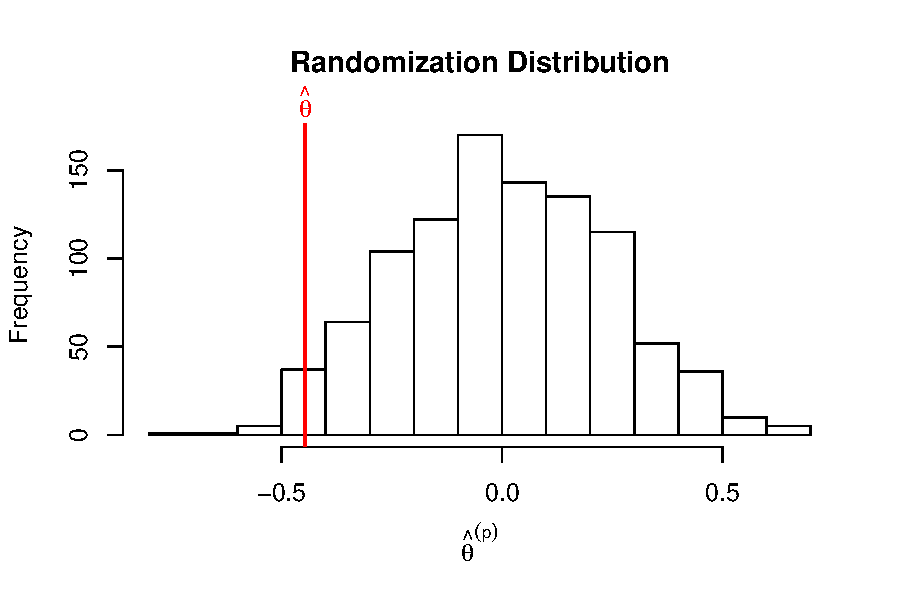
\includegraphics[width=\maxwidth]{figure/plot_test-1} 

}



\end{knitrout}

More generally, we could have equivalently used the function \texttt{permtest()} for this analysis
\begin{knitrout}
\definecolor{shadecolor}{rgb}{0.969, 0.969, 0.969}\color{fgcolor}\begin{kframe}
\begin{alltt}
\hlstd{m1} \hlkwb{<-} \hlkwd{glm}\hlstd{(bpepisodes} \hlopt{~} \hlstd{spnvac,} \hlkwc{family} \hlstd{= poisson,} \hlkwc{data} \hlstd{= pneumovac)}
\hlstd{test} \hlkwb{<-} \hlkwd{permtest}\hlstd{(m1,} \hlkwc{trtname} \hlstd{=} \hlstr{'spnvac'}\hlstd{,} \hlkwc{runit} \hlstd{=} \hlstr{'randunit'}\hlstd{,}
                 \hlkwc{data} \hlstd{= pneumovac,} \hlkwc{nperm} \hlstd{=} \hlnum{1000}\hlstd{,} \hlkwc{ncores} \hlstd{=} \hlnum{1}\hlstd{,} \hlkwc{seed} \hlstd{=} \hlnum{444}\hlstd{)}
\hlkwd{print}\hlstd{(}\hlkwd{c}\hlstd{(}\hlkwd{exp}\hlstd{(test}\hlopt{$}\hlstd{coef), test}\hlopt{$}\hlstd{pval))} \hlcom{# IRR}
\end{alltt}
\begin{verbatim}
## [1] 0.6397397 0.0580000
\end{verbatim}
\end{kframe}
\end{knitrout}
\noindent The \texttt{model} (first argument) must correspond to a regression model that accomodates an offset term and one for which coefficients can be extracted in the standard way (i.e. using \texttt{coef()}). For example, it can be an object of class \texttt{"glm"}, \texttt{"survreg"}, \texttt{"coxph"}, etc.

\subsection{Randomization-Based Confidence Interval}
\label{ci}
Now let's get the corresponding randomization-based 95\% CI using \texttt{permci\_glm()}.
\begin{knitrout}
\definecolor{shadecolor}{rgb}{0.969, 0.969, 0.969}\color{fgcolor}\begin{kframe}
\begin{alltt}
\hlstd{ci} \hlkwb{<-} \hlkwd{permci_glm}\hlstd{(bpepisodes} \hlopt{~} \hlstd{spnvac,} \hlkwc{trtname} \hlstd{=} \hlstr{'spnvac'}\hlstd{,}
                 \hlkwc{runit} \hlstd{=} \hlstr{'randunit'}\hlstd{,} \hlkwc{family} \hlstd{= poisson,} \hlkwc{data} \hlstd{= pneumovac,}
                 \hlkwc{nperm} \hlstd{=} \hlnum{1000}\hlstd{,} \hlkwc{ncores} \hlstd{=} \hlnum{2}\hlstd{,} \hlkwc{seed} \hlstd{=} \hlnum{445}\hlstd{,} \hlkwc{level} \hlstd{=} \hlnum{0.95}\hlstd{,}
                 \hlkwc{initmethod} \hlstd{=} \hlstr{'perm'}\hlstd{)}
\hlkwd{print}\hlstd{(ci}\hlopt{$}\hlstd{ci)} \hlcom{# logIRR}
\end{alltt}
\begin{verbatim}
##       lower       upper 
## -0.97314014  0.06265964
\end{verbatim}
\begin{alltt}
\hlkwd{print}\hlstd{(}\hlkwd{exp}\hlstd{(ci}\hlopt{$}\hlstd{ci))} \hlcom{# IRR}
\end{alltt}
\begin{verbatim}
##     lower     upper 
## 0.3778945 1.0646644
\end{verbatim}
\end{kframe}
\end{knitrout}
\noindent Most of the arguments are the same except the additional specification of the confidence \texttt{level} (95\% here) and \texttt{initmethod}, which specifies the method to obtain initial values for the CI procedure (see \texttt{?permci\_glm} for more detail). If \texttt{ncores} $>$ 1 for \texttt{permci\_glm()}, lower and upper bound search procedures run in parallel across two cores (but not more than two).

We get a 95\% CI for the IRR of 0.38 to 1.06. The CI is calculated using an efficient search procedure adapted from Garthwaite (1996), with \texttt{method = "G"} (default), or the procedure adapted from Garthwaite and Jones (2009), with \texttt{method = "GJ"}(see Section~\ref{GJ}). We can inspect convergence of each bound simply by using \texttt{plot(ci)}:
\begin{knitrout}
\definecolor{shadecolor}{rgb}{0.969, 0.969, 0.969}\color{fgcolor}

{\centering 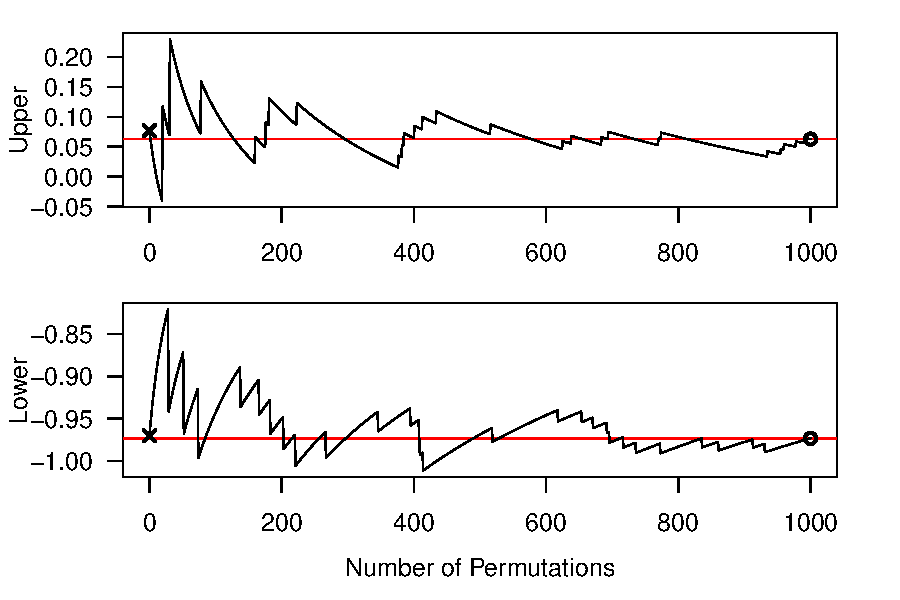
\includegraphics[width=\maxwidth]{figure/plot_ci-1} 

}



\end{knitrout}
\noindent Note: we've used only 1,000 permutations in this example for convenience. In practice, we'll usually need to increase the number of permutations to ensure adequate approximation of the exact p-value and convergence of the CI bounds.

Again, we could have equivalently used the function \texttt{permci()} for this analysis
\begin{knitrout}
\definecolor{shadecolor}{rgb}{0.969, 0.969, 0.969}\color{fgcolor}\begin{kframe}
\begin{alltt}
\hlstd{ci} \hlkwb{<-} \hlkwd{permci}\hlstd{(m1,} \hlkwc{trtname} \hlstd{=} \hlstr{'spnvac'}\hlstd{,} \hlkwc{runit} \hlstd{=} \hlstr{'randunit'}\hlstd{,} \hlkwc{data} \hlstd{= pneumovac,}
             \hlkwc{nperm} \hlstd{=} \hlnum{1000}\hlstd{,} \hlkwc{ncores} \hlstd{=} \hlnum{2}\hlstd{,} \hlkwc{seed} \hlstd{=} \hlnum{445}\hlstd{)}
\hlkwd{print}\hlstd{(}\hlkwd{exp}\hlstd{(ci}\hlopt{$}\hlstd{ci))} \hlcom{# IRR}
\end{alltt}
\begin{verbatim}
##     lower     upper 
## 0.3778945 1.0646644
\end{verbatim}
\end{kframe}
\end{knitrout}

\section{Going a Bit Deeper}

\subsection{Stratified Randomization}
CRTs often employ stratified randomization to improve balance between treatment arms, which can increase the power of the trial. Stratified designs can be accomodated simply by restricting the set of permutations considered. In \textbf{permuter}, this just means including one additional argument, \texttt{strat}, when calling the test or CI function of interest.

To illustrate this, let's consider the Botswana Combination Prevention Project (BCPP), a pair-matched HIV prevention CRT to test whether a combination treatment and prevention intervention could reduce population-level cumulative HIV incidence over 3 years of follow-up. A total of 30 communities were randomized, 15 to each arm. The primary study endpoint was cumulative HIV incidence, measured at scheduled study visits as time to HIV-infection within a cohort of individuals identified as HIV-negative among a 20\% random sample of eligible households at baseline. That is, we have an interval-censored time-to-event outcome for each cohort participant. Since the primary trial data are confidential, we use a simulated data set, which was generated to mimic the BCPP by applying an agent-based epidemic model to a dynamic network of simulated sexual partnerships (Goyal, Blitzstein, and De Gruttola, 2013; Wang et al., 2014). These data are also available in the \textbf{permuter} package.

The \texttt{bcpp} data frame contains an indicator for assigment to the intervention arm (\texttt{treat}), a distinct identifier for community (\texttt{group}) and matched pair (\texttt{pair.id}), and two columns representing the interval-censored time-to-event outcome (\texttt{left}, \texttt{right}) measured in weeks.
\begin{knitrout}
\definecolor{shadecolor}{rgb}{0.969, 0.969, 0.969}\color{fgcolor}\begin{kframe}
\begin{alltt}
\hlkwd{head}\hlstd{(bcpp)}
\end{alltt}
\begin{verbatim}
##   group pair.id treat     left right
## 1     1       1     0 154.9326   Inf
## 2     1       1     0 155.4123   Inf
## 3     1       1     0 156.9418   Inf
## 4     1       1     0 152.7263   Inf
## 5     1       1     0 155.7767   Inf
## 6     1       1     0 159.4207   Inf
\end{verbatim}
\end{kframe}
\end{knitrout}
Let's carry out randomization-based inference for these data, making sure we restrict the analysis based on the pair-matched design by including \texttt{strat = "pair.id"}. We'll use the estimated treatment effect from an interval-censored Weibull regression model as our test statistic.
\begin{knitrout}
\definecolor{shadecolor}{rgb}{0.969, 0.969, 0.969}\color{fgcolor}\begin{kframe}
\begin{alltt}
\hlkwd{library}\hlstd{(survival)}
\hlstd{m1} \hlkwb{<-} \hlkwd{survreg}\hlstd{(}\hlkwd{Surv}\hlstd{(left, right,} \hlkwc{type} \hlstd{=} \hlstr{'interval2'}\hlstd{)} \hlopt{~} \hlstd{treat,} \hlkwc{data} \hlstd{= bcpp)}
\hlstd{test} \hlkwb{<-} \hlkwd{permtest}\hlstd{(m1,} \hlkwc{trtname} \hlstd{=} \hlstr{'treat'}\hlstd{,} \hlkwc{runit} \hlstd{=} \hlstr{'group'}\hlstd{,}
                 \hlkwc{strat} \hlstd{=} \hlstr{'pair.id'}\hlstd{,} \hlkwc{data} \hlstd{= bcpp,}
                 \hlkwc{nperm} \hlstd{=} \hlnum{10}\hlstd{,} \hlkwc{ncores} \hlstd{=} \hlnum{3}\hlstd{,} \hlkwc{seed} \hlstd{=} \hlnum{446}\hlstd{)}
\hlstd{ci} \hlkwb{<-} \hlkwd{permci}\hlstd{(m1,} \hlkwc{trtname} \hlstd{=} \hlstr{'treat'}\hlstd{,} \hlkwc{runit} \hlstd{=} \hlstr{'group'}\hlstd{,}
             \hlkwc{strat} \hlstd{=} \hlstr{'pair.id'}\hlstd{,} \hlkwc{data} \hlstd{= bcpp,}
             \hlkwc{nperm} \hlstd{=} \hlnum{10}\hlstd{,} \hlkwc{ncores} \hlstd{=} \hlnum{2}\hlstd{,} \hlkwc{seed} \hlstd{=} \hlnum{447}\hlstd{)}
\hlkwd{print}\hlstd{(}\hlkwd{c}\hlstd{(test}\hlopt{$}\hlstd{coef, test}\hlopt{$}\hlstd{pval))}
\end{alltt}
\begin{verbatim}
## [1] 0.5030926 0.1000000
\end{verbatim}
\begin{alltt}
\hlkwd{print}\hlstd{(ci}\hlopt{$}\hlstd{ci)}
\end{alltt}
\begin{verbatim}
##     lower     upper 
## 0.2249209 0.7848803
\end{verbatim}
\begin{alltt}
\hlcom{# Transform Weibull AFT to PH, i.e. estimated hazard ratio}
\hlkwd{print}\hlstd{(}\hlkwd{c}\hlstd{(}\hlkwd{exp}\hlstd{(}\hlopt{-}\hlstd{test}\hlopt{$}\hlstd{coef} \hlopt{/} \hlstd{m1}\hlopt{$}\hlstd{scale), test}\hlopt{$}\hlstd{pval))}
\end{alltt}
\begin{verbatim}
## [1] 0.5875714 0.1000000
\end{verbatim}
\begin{alltt}
\hlkwd{print}\hlstd{(}\hlkwd{as.numeric}\hlstd{(}\hlkwd{rev}\hlstd{(}\hlkwd{exp}\hlstd{(}\hlopt{-}\hlstd{ci}\hlopt{$}\hlstd{ci} \hlopt{/} \hlstd{m1}\hlopt{$}\hlstd{scale))))}
\end{alltt}
\begin{verbatim}
## [1] 0.4362234 0.7884105
\end{verbatim}
\end{kframe}
\end{knitrout}
\noindent These results suggest better outcomes (i.e. reduced hazard of HIV-infection) among those living in communities randomized to the intervention. Note, we didn't explicitly set \texttt{level = 0.95} or \texttt{initmethod = "perm"} this time, but these are the default values.

Matching and stratification are just special forms of \textit{restricted} randomization, which is also handled by restricting the set of permutations in the analysis. We plan to implement this more general functionality in future versions of \textbf{permuter}.

\subsection{Fine-Tuning the Confidence Interval}
The efficient CI algorithm (Garthwaite, 1996) used in \textbf{permuter} substantially reduces the computational burden of obtaining randomization-based CIs, but its performance could be affected by some of the choices that have been made under the hood. For example, one may wish to consider different starting values, restart the algorithm if the starting values seem poor, or modify the magnitude of each step in the algorithm. Let's see how we can fine-tune our CIs in \textbf{permuter}.

Let's generate some data from a CRT with a binary outcome.
\begin{knitrout}
\definecolor{shadecolor}{rgb}{0.969, 0.969, 0.969}\color{fgcolor}\begin{kframe}
\begin{alltt}
\hlstd{ds} \hlkwb{<-} \hlkwd{gendata_crt}\hlstd{(}\hlkwc{family} \hlstd{= binomial,} \hlkwc{nclus} \hlstd{=} \hlkwd{c}\hlstd{(}\hlnum{10}\hlstd{,} \hlnum{10}\hlstd{),} \hlkwc{size} \hlstd{=} \hlkwd{c}\hlstd{(}\hlnum{30}\hlstd{,} \hlnum{50}\hlstd{),}
                  \hlkwc{theta} \hlstd{=} \hlkwd{log}\hlstd{(}\hlnum{1.5}\hlstd{),} \hlkwc{mu} \hlstd{=} \hlkwd{qlogis}\hlstd{(}\hlnum{0.25}\hlstd{),} \hlkwc{sigma} \hlstd{=} \hlnum{0.2}\hlstd{)}
\hlkwd{dim}\hlstd{(ds)}
\end{alltt}
\begin{verbatim}
## [1] 786   5
\end{verbatim}
\begin{alltt}
\hlkwd{head}\hlstd{(ds)}
\end{alltt}
\begin{verbatim}
##   unique.id clusid id trt y
## 1       1.1      1  1   1 0
## 2       1.2      1  2   1 0
## 3       1.3      1  3   1 0
## 4       1.4      1  4   1 0
## 5       1.5      1  5   1 1
## 6       1.6      1  6   1 0
\end{verbatim}
\end{kframe}
\end{knitrout}
\noindent We've created a data set with 10 clusters in each study arm, ranging in size from 30 to 50 individuals. Other arguments control the true underlying treatment effect (e.g. an odds ratio of 1.5), the prevalence the outcome in the control group (e.g. 25\%), and the level of between-cluster hetergeneity (see \texttt{?gendata\_crt} for more details).

Let's compute four CIs with different sets of starting values: the first based on a small permutation test, the second based on a naive asymptotic CI, and the last two specifying the initial values ourselves.
\begin{knitrout}
\definecolor{shadecolor}{rgb}{0.969, 0.969, 0.969}\color{fgcolor}\begin{kframe}
\begin{alltt}
\hlstd{nperm} \hlkwb{<-} \hlnum{500}
\hlstd{ci1} \hlkwb{<-} \hlkwd{permci_glm}\hlstd{(y} \hlopt{~} \hlstd{trt,} \hlkwc{trtname} \hlstd{=} \hlstr{'trt'}\hlstd{,} \hlkwc{runit} \hlstd{=} \hlstr{'clusid'}\hlstd{,}
                  \hlkwc{family} \hlstd{= binomial,} \hlkwc{data} \hlstd{= ds,} \hlkwc{nperm} \hlstd{= nperm,} \hlkwc{ncores} \hlstd{=} \hlnum{2}\hlstd{,}
                  \hlkwc{seed} \hlstd{=} \hlnum{448}\hlstd{,} \hlkwc{initmethod} \hlstd{=} \hlstr{'perm'}\hlstd{)}
\hlstd{ci2} \hlkwb{<-} \hlkwd{permci_glm}\hlstd{(y} \hlopt{~} \hlstd{trt,} \hlkwc{trtname} \hlstd{=} \hlstr{'trt'}\hlstd{,} \hlkwc{runit} \hlstd{=} \hlstr{'clusid'}\hlstd{,}
                  \hlkwc{family} \hlstd{= binomial,} \hlkwc{data} \hlstd{= ds,} \hlkwc{nperm} \hlstd{= nperm,} \hlkwc{ncores} \hlstd{=} \hlnum{2}\hlstd{,}
                  \hlkwc{seed} \hlstd{=} \hlnum{449}\hlstd{,} \hlkwc{initmethod} \hlstd{=} \hlstr{'asymp'}\hlstd{)}
\hlstd{ci3} \hlkwb{<-} \hlkwd{permci_glm}\hlstd{(y} \hlopt{~} \hlstd{trt,} \hlkwc{trtname} \hlstd{=} \hlstr{'trt'}\hlstd{,} \hlkwc{runit} \hlstd{=} \hlstr{'clusid'}\hlstd{,}
                  \hlkwc{family} \hlstd{= binomial,} \hlkwc{data} \hlstd{= ds,} \hlkwc{nperm} \hlstd{= nperm,} \hlkwc{ncores} \hlstd{=} \hlnum{2}\hlstd{,}
                  \hlkwc{seed} \hlstd{=} \hlnum{450}\hlstd{,} \hlkwc{init} \hlstd{=} \hlkwd{c}\hlstd{(}\hlopt{-}\hlnum{1}\hlstd{,} \hlnum{2}\hlstd{))}
\hlstd{ci4} \hlkwb{<-} \hlkwd{permci_glm}\hlstd{(y} \hlopt{~} \hlstd{trt,} \hlkwc{trtname} \hlstd{=} \hlstr{'trt'}\hlstd{,} \hlkwc{runit} \hlstd{=} \hlstr{'clusid'}\hlstd{,}
                  \hlkwc{family} \hlstd{= binomial,} \hlkwc{data} \hlstd{= ds,} \hlkwc{nperm} \hlstd{= nperm,} \hlkwc{ncores} \hlstd{=} \hlnum{2}\hlstd{,}
                  \hlkwc{seed} \hlstd{=} \hlnum{451}\hlstd{,} \hlkwc{init} \hlstd{=} \hlkwd{c}\hlstd{(}\hlopt{-}\hlnum{2}\hlstd{,} \hlnum{3}\hlstd{))}
\end{alltt}
\end{kframe}
\end{knitrout}

\begin{knitrout}
\definecolor{shadecolor}{rgb}{0.969, 0.969, 0.969}\color{fgcolor}

{\centering 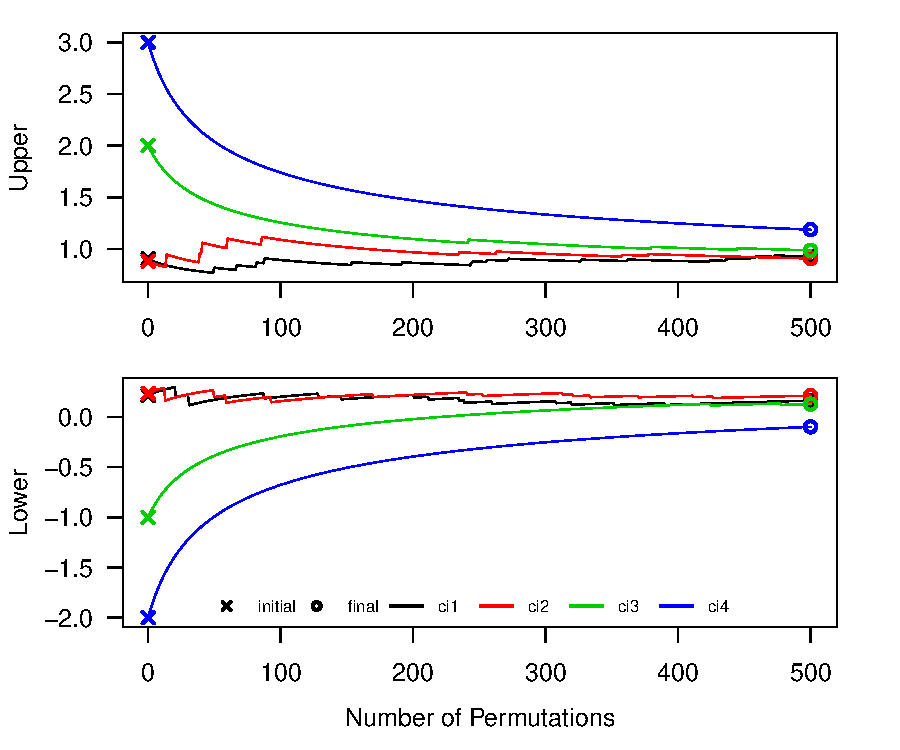
\includegraphics[width=\maxwidth]{figure/ci_plots-1} 

}



\end{knitrout}
\noindent We see that \texttt{ci4} resulted in the widest CI, suggesting this search was sensitive to the wide starting values. Increasing the number of permutations may mitigate this sensitivity.

Another approach we could use to combat poor starting values is restarting the algorithm after a fixed number of permutations. Since the magnitude of the steps gets smaller as the search proceeds, it may take a large number of permutations to recover from bad starting values. Using a ``burn-in'' phase can speed up its recovery. Let's consider the same four sets of starting values as before, but now specify the additional argument \texttt{nburn = 100}.


\begin{knitrout}
\definecolor{shadecolor}{rgb}{0.969, 0.969, 0.969}\color{fgcolor}

{\centering 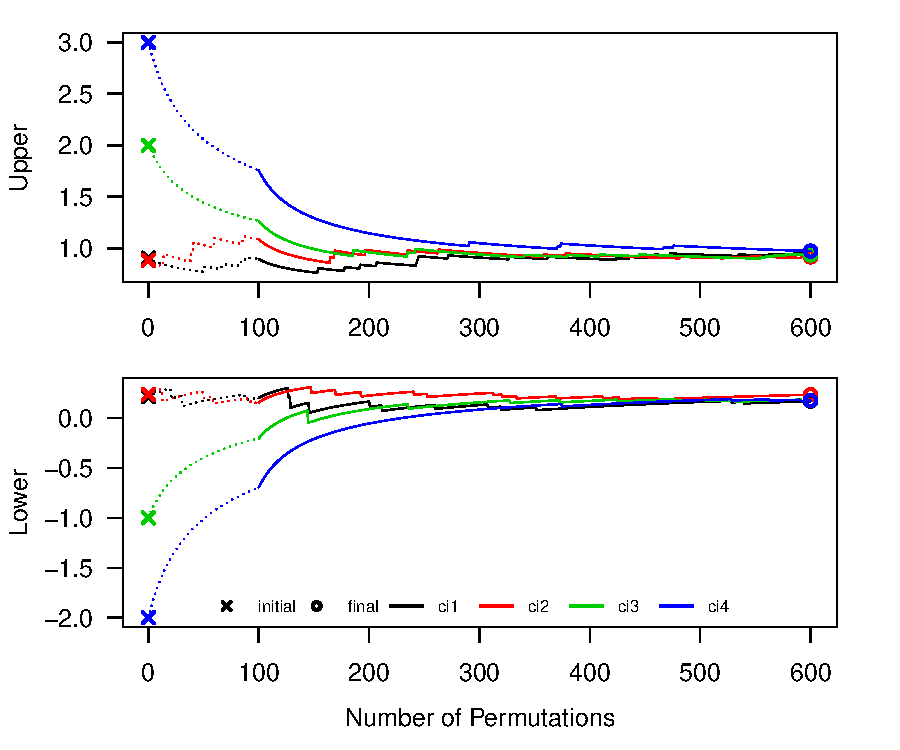
\includegraphics[width=\maxwidth]{figure/ci_plots2-1} 

}



\end{knitrout}
\noindent Comparing back to the plot without the burn-in permutations, our final estimates are much less sensitive to the poor initial values of \texttt{ci3} and \texttt{ci4}. Even if we had fixed the total number of permutations at 500 and stopped after 400 post-burn-in permutations, we would have done better than before.

We can go even deeper by modifying the search algorithm itself. For example, we can specify \texttt{permci\_glm(..., m = 1)} to set the largest initial step magnitude (the magnitude is inversely proportional to \texttt{m}). This is yet another approach that may speed up convergence if we choose poor starting values, but could introduce problems if the first few steps happen to jump even further away from the true bounds. Below, we see improved convergence by using a larger initial step size.


\begin{knitrout}
\definecolor{shadecolor}{rgb}{0.969, 0.969, 0.969}\color{fgcolor}

{\centering 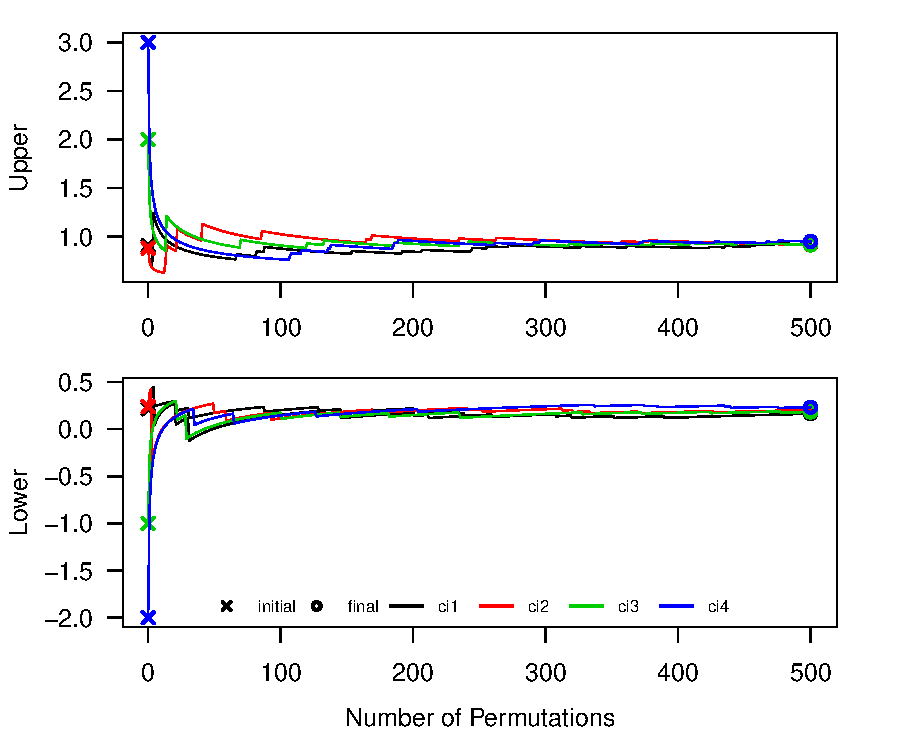
\includegraphics[width=\maxwidth]{figure/ci_plots3-1} 

}



\end{knitrout}

\subsection{Alternative Procedure for Longer CI Searches}
\label{GJ}

For longer searches (e.g. \texttt{nperm >= 200,000}), Garthwaite and Jones (2009) proposed an improvement on the algorithm in Garthwaite (1996) by taking larger steps during later phases of the search and averaging, rather than using only the final values, for CI estimation. This alternative procedure can be used by specifying \texttt{permci\_glm(..., method = "GJ")}. Here we use this alternative procedure with \texttt{nperm = 1000} just for illustration. Compare this back to the search in Section~\ref{ci}.
\begin{knitrout}
\definecolor{shadecolor}{rgb}{0.969, 0.969, 0.969}\color{fgcolor}\begin{kframe}
\begin{alltt}
\hlstd{ci} \hlkwb{<-} \hlkwd{permci_glm}\hlstd{(bpepisodes} \hlopt{~} \hlstd{spnvac,} \hlkwc{trtname} \hlstd{=} \hlstr{'spnvac'}\hlstd{,}
                 \hlkwc{runit} \hlstd{=} \hlstr{'randunit'}\hlstd{,} \hlkwc{family} \hlstd{= poisson,} \hlkwc{data} \hlstd{= pneumovac,}
                 \hlkwc{nperm} \hlstd{=} \hlnum{1000}\hlstd{,} \hlkwc{ncores} \hlstd{=} \hlnum{2}\hlstd{,} \hlkwc{seed} \hlstd{=} \hlnum{445}\hlstd{,} \hlkwc{method} \hlstd{=} \hlstr{'GJ'}\hlstd{)}
\hlkwd{print}\hlstd{(ci}\hlopt{$}\hlstd{ci)} \hlcom{# logIRR}
\end{alltt}
\begin{verbatim}
##       lower       upper 
## -0.96278337  0.04988705
\end{verbatim}
\begin{alltt}
\hlkwd{print}\hlstd{(}\hlkwd{exp}\hlstd{(ci}\hlopt{$}\hlstd{ci))} \hlcom{# IRR}
\end{alltt}
\begin{verbatim}
##     lower     upper 
## 0.3818286 1.0511524
\end{verbatim}
\begin{alltt}
\hlkwd{plot}\hlstd{(ci)}
\end{alltt}
\end{kframe}

{\centering 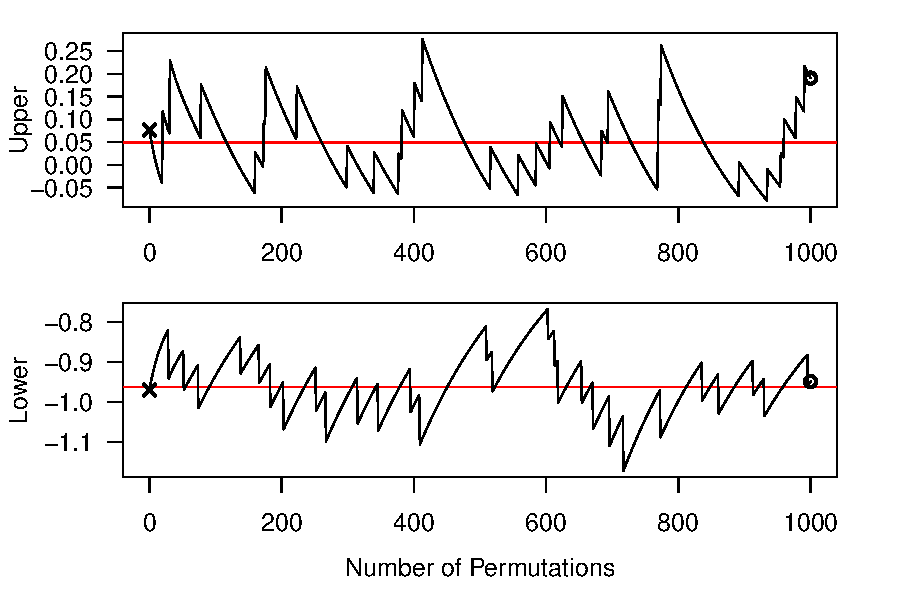
\includegraphics[width=\maxwidth]{figure/pci3-1} 

}



\end{knitrout}

\section*{Contact}
For more information or to report any issues, please email \href{mailto:djrabideau@mail.harvard.edu}{djrabideau@mail.harvard.edu}.

\section*{References}
\noindent\hangindent=15pt Dwass, M. (1957). Modified Randomization Tests for Nonparametric Hypotheses. \textit{The Annals of Mathematical Statistics} \textbf{28}, 181--187.

\noindent\hangindent=15pt Garthwaite, P. H. (1996). Confidence intervals from randomization tests. \textit{Biometrics} \textbf{52}, 1387--1393.

\noindent\hangindent=15pt Garthwaite, P. H. and Buckland, S. T. (1992). Generating Monte Carlo Confidence Intervals by the Robbins-Monro Process. \textit{Journal of the Royal Statistical Society. Series C (Applied Statistics)} \textbf{41}, 159--171.

\noindent\hangindent=15pt Garthwaite, P. H. and Jones, M. C. (2009). A Stochastic Approximation Method and Its Application to Confidence Intervals. \textit{Journal of Computational and Graphical Statistics} \textbf{18}, 184--200.

\noindent\hangindent=15pt Goyal, R., Blitzstein, J., and De Gruttola, V. (2013). Simulating Bipartite Networks to Reflect Uncertainty in Local Network Properties. \textit{Harvard University Biostatistics Working Paper Series}.

\noindent\hangindent=15pt Hayes, R. J. and Moulton, L. H. (2017). \textit{Cluster Randomised Trials} 2nd edition. New York: Chapman and Hall/CRC.

\noindent\hangindent=15pt O'Brien, K. L. et al. (2003). Efficacy and safety of seven-valent conjugate pneumococcal vaccine in American Indian children: group randomised trial. \textit{Lancet} \textbf{362}, 355--361.

\noindent\hangindent=15pt Rabideau, D. J., and Wang, R. Randomization-Based Confidence Intervals for Cluster Randomized Trials. Under Review.

\noindent\hangindent=15pt Wang, R., Goyal, R., Lei, Q., Essex, M., and De~Gruttola, V. (2014). Sample size considerations in the design of cluster randomized trials of combination HIV prevention. \textit{Clinical Trials} \textbf{11}, 309--318.

\end{document}
